\section{模型架构与方法}
\subsection{数据准备}
\subsubsection{语料准备}

语料的选择为谭松波老师的评论语料\cite{hotel-comment},正负例各2000。属于较小的数据集,本项目包含了原始语料。将原本gb2312编码文件转换成utf-8编码的文件。

\subsubsection{词向量准备}

本实验使用开源词向量chinese-word-vectors\cite{P18-2023},选择知乎语料训练而成的Word Vector。

\subsection{基于CNN实现}
\subsubsection{CNN基本结构}
卷积神经网络(Convolutional Neural Network, CNN)是一种深度学习模型,特别擅长处理具有网格拓扑结构的数据。CNN 由多个层(layers)组成,每一层执行特定的功能。主要包括以下几种层:
\begin{enumerate}
    \item \textbf{输入层(Input Layer)}\newline
    通常是一个三维数组(高度 × 宽度 × 通道)
    \item \textbf{卷积层(Convolutional Layer)}
    \begin{itemize}
        \item 通过卷积核(filters)对输入进行卷积操作,提取局部特征。每个卷积核在输入图像上滑动,执行点积运算,生成特征图(feature map)
        \item 卷积操作公式:
        \begin{equation}
            (I \ast K)(x, y) = \sum_m \sum_n I(m, n) \cdot K(x - m, y - n)
        \end{equation}
        其中,\( I \) 是输入,\( K \) 是卷积核,\((x, y)\) 是输出特征图的位置
        \item 填充(Padding)
        \begin{itemize}
            \item Valid Padding: 不使用填充,卷积会导致输出尺寸减小
            \item Same Padding: 使用填充,使输出尺寸与输入相同
        \end{itemize}
        \item 步幅(Stride)\newline
        卷积核在输入图像上滑动的步长。步幅越大,输出特征图尺寸越小。
    \end{itemize}
    \item \textbf{激活层(Activation Layer)}
    \begin{itemize}
        \item 通常使用 ReLU(Rectified Linear Unit)激活函数,将非线性引入模型
        \item 公式:
        \begin{equation}
            f(x) = \max(0, x)
        \end{equation}
        其他常见的激活函数包括 Sigmoid、Tanh 等
    \end{itemize}
    \item \textbf{池化层(Pooling Layer)}\newline
    池化层通过下采样操作(如最大池化或平均池化)减少特征图的尺寸,降低计算量和参数量,同时保留重要特征。
    \begin{itemize}
        \item 最大池化公式:
        \begin{equation}
            y = \max(x_i)
        \end{equation}
        \item 平均池化公式:
        \begin{equation}
            y = \frac{1}{n} \sum_{i=1}^{n} x_i
        \end{equation}
    \end{itemize}
    \item \textbf{全连接层(Fully Connected Layer)}\newline
    全连接层将前一层的特征展平成一维向量,与权重矩阵相乘并加上偏置,进行分类或回归任务。\newline
    全连接层公式:
    \begin{equation}
        y = Wx + b
    \end{equation}
    \item \textbf{输出层(Output Layer)}\newline
    输出层根据任务的不同可以使用不同的激活函数。例如,softmax 激活函数用于多分类任务,sigmoid 用于二分类任务。
\end{enumerate}
\subsubsection{基于CNN的中文情感分析模型}

根据Zhang, Ye等人\cite{zhang2015sensitivity}的关于CNN的情感分析的研究和相关博客\cite{CNN-text-classification-tf},实现了我们的基于CNN的中文情感分析模型。模型的架构如图\ref{fig:CNN}所示。

首先,我们采用了基于预训练词向量的单通道,将语料进行Embedding后,输入给带有多层滤波器和特征如的卷积神经网络。这里我们实现了多个不同长度的定宽卷积核。

随后,将CNN网络的输出传给最大池化层,对每个滤波器的输出仅取一个最大值。

最后,输入给带有Dropout和Softmax的全连接层,得到最终模型输出。经过Softmax操作,我们得到了对输入语句的情感分析结果(积极-POS,消极-NEG)的概率。

对于模型实现的细节,我们在代码实现部分进行了详细分析。

\begin{figure}[H]
    \centering
    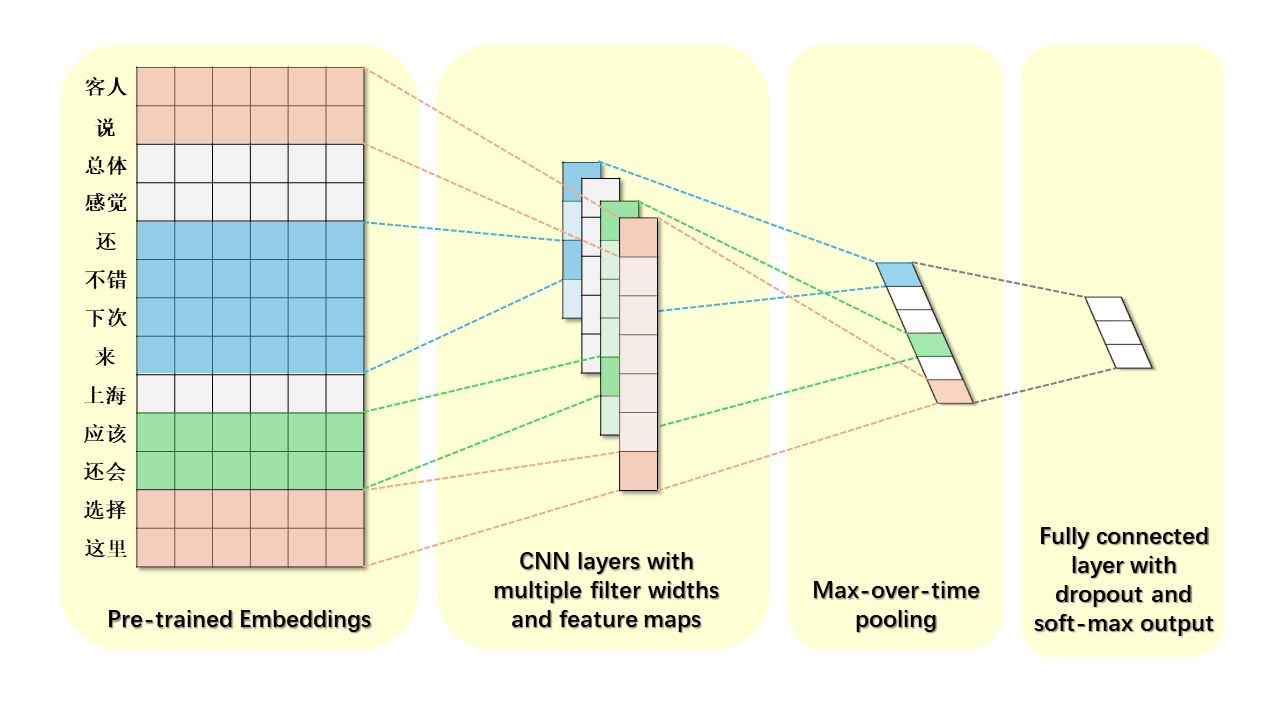
\includegraphics[width=1.0\linewidth]{sections//fig/cnn.png}
    \caption{基于CNN的中文情感分析}
    \label{fig:CNN}
\end{figure}

\subsection{基于BiLSTM实现}
\subsubsection{BiLSTM基本结构}
双向长短期记忆网络(Bidirectional Long Short-Term Memory,BiLSTM)是一种用于处理序列数据的深度学习模型,广泛应用于自然语言处理任务中,如情感分析、机器翻译和语音识别等。
\begin{enumerate}
    \item \textbf{LSTM单元}\newline
    LSTM单元是BiLSTM的基本构建模块。标准的RNN容易在处理长序列时遗忘前面的信息,而LSTM通过引入记忆单元(Cell State)和三个门控机制(输入门、遗忘门、输出门)来有效缓解这一问题。LSTM单元在每个时间步的计算如下:
    \begin{itemize}
        \item \textbf{遗忘门(Forget Gate):}决定需要遗忘的上一个时间步的信息。计算公式如下:\newline
        \begin{equation}
            f_t = \sigma(W_f \cdot [h_{t-1}, x_t] + b_f)
        \end{equation}
        其中,$\sigma$ 是Sigmoid激活函数,$W_f$ 是权重矩阵,$h_{t-1}$ 是上一个时间步的隐藏状态,$x_t$ 是当前时间步的输入,$b_f$ 是偏置项。
        \item \textbf{输入门(Input Gate):}决定新的信息要更新到记忆单元中的哪些部分。计算公式如下:
        \begin{equation}
            i_t = \sigma(W_i \cdot [h_{t-1}, x_t] + b_i)
        \end{equation}
        \begin{equation}
            \tilde{C}_t = \tanh(W_C \cdot [h_{t-1}, x_t] + b_C)
        \end{equation}
其中,$\tanh$ 是双曲正切激活函数,$W_i$ 和 $W_C$ 是权重矩阵,$b_i$ 和 $b_C$ 是偏置项,$\tilde{C}_t$ 是新的候选记忆单元状态。
        \item \textbf{记忆单元更新:}结合遗忘门和输入门的信息,更新记忆单元状态。计算公式如下:
        \begin{equation}
            C_t = f_t \cdot C_{t-1} + i_t \cdot \tilde{C}_t
        \end{equation}
        \item \textbf{输出门(Output Gate):}决定隐藏状态的输出。计算公式如下:
        \begin{equation}
            o_t = \sigma(W_o \cdot [h_{t-1}, x_t] + b_o)
        \end{equation}
        \begin{equation}
            h_t = o_t \cdot \tanh(C_t)
        \end{equation}
    \end{itemize}
    在这些公式中,$C_t$ 是记忆单元的状态,$h_t$ 是隐藏状态。
    \item \textbf{双向机制}\newline
    BiLSTM通过结合正向和反向的LSTM层,进一步增强模型对上下文信息的捕捉能力。
    \begin{itemize}
        \item \textbf{正向LSTM:}从序列的前向后处理数据,生成正向隐藏状态序列 $\overrightarrow{h_t}$:
        \begin{equation}
            \overrightarrow{h_t} = \text{LSTM}(x_t, \overrightarrow{h_{t-1}}, \overrightarrow{C_{t-1}})
        \end{equation}
        \item \textbf{反向LSTM:}从序列的后向前处理数据,生成反向隐藏状态序列 $\overleftarrow{h_t}$:
        \begin{equation}
            \overleftarrow{h_t} = \text{LSTM}(x_t, \overleftarrow{h_{t+1}}, \overleftarrow{C_{t+1}})
        \end{equation}
    \end{itemize}
    在每个时间步t,正向隐藏状态和反向隐藏状态会被连接起来,形成最终的隐藏状态 $h_t$:
    \begin{equation}
        h_t = [\overrightarrow{h_t}; \overleftarrow{h_t}]
    \end{equation}

\end{enumerate}
\subsubsection{基于BiLSTM的中文情感分析模型}

BiLSTM在自然语言处理领域展示着优越的性能\cite{huang2015bidirectional}。ELMo\cite{sarzynska2021detecting}使用了BiLSTM作为模型的基础,展示了在情感分析和其他 NLP 任务上的卓越表现。不难发现,BiLSTM通过捕捉全面的上下文信息、处理长距离依赖关系、适应多样化的句子结构以及对抗文本噪声等优势,使其在情感分析任务中表现优异。所以,我们尝试使用BiLSTM模型处理中文情感分析。

基于BI-LSTM模型的中文情感分析模型有如下步骤:

\begin{itemize}[noitemsep, topsep=1pt, partopsep=1pt, parsep=1pt, left=32pt]
    \item 中文词嵌入层。
    \item 使用BI-LSTM模型。
    \item 带有Softmax的全连接。
\end{itemize}

\vspace{8pt}

基于BiLSTM的中文情感分析的模型架构如图\ref{fig:bilstm}所示。

\vspace{8pt}

\begin{figure}[H]
    \centering
    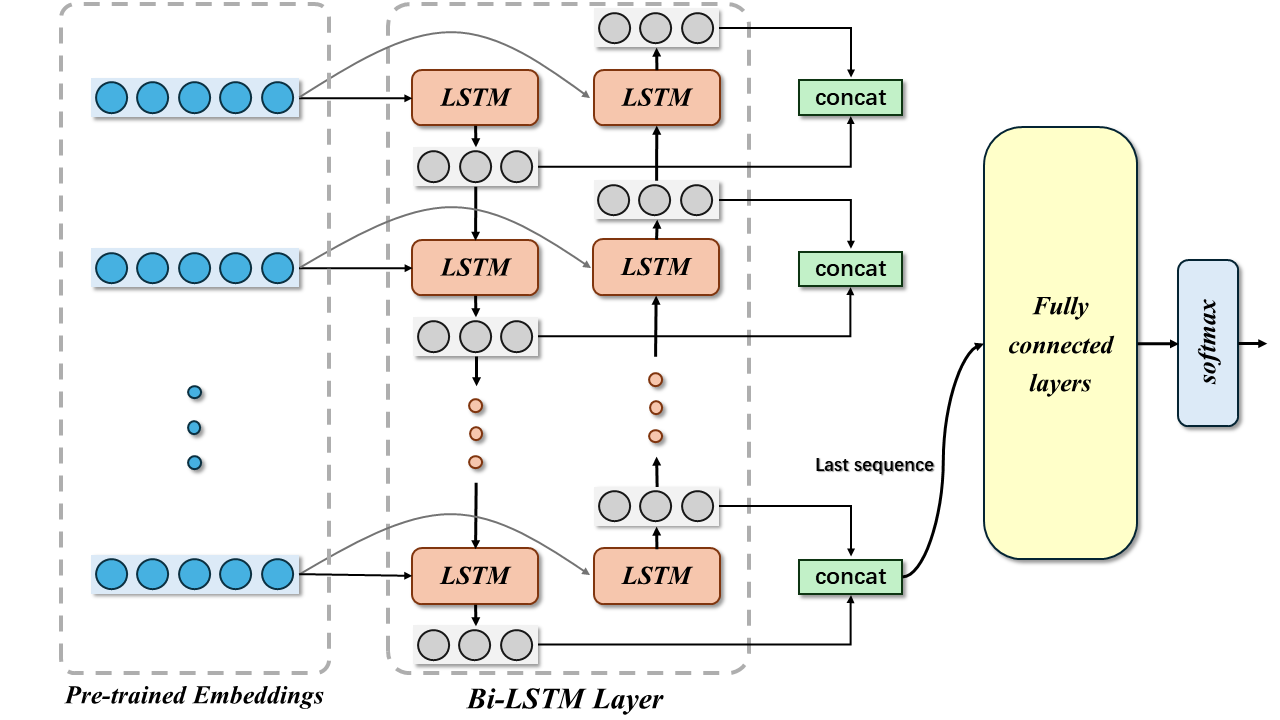
\includegraphics[width=1.0\linewidth]{sections//fig/bilstm.png}
    \caption{基于BI-LSTM的中文情感分析}
    \label{fig:bilstm}
\end{figure}

对于模型实现的细节,我们在代码实现部分进行了详细分析。